% %% %%%%%%%%%%%%%%%%%%%%%%%%%%%%%%%%%%%%%%%%%%%%%%%%%%%%%%%%%%
% steps.tex
%
% Author:  Mauricio Matamoros
% License: MIT
%
% %% %%%%%%%%%%%%%%%%%%%%%%%%%%%%%%%%%%%%%%%%%%%%%%%%%%%%%%%%%%

%!TEX root = ../practica.tex
%!TEX root = ../references.bib

\section{Instrucciones}%
\label{sec:instructions}
\begin{enumerate}[noitemsep]
	\item Configure su entorno de desarrollo tomando siguiendo los pasos de la \Cref{sec:step1}.
	\item Descargue y configure buildroot como se describe en las \Cref{sec:step2,sec:step3}.
	\item Siguiendo los pasos de la \Cref{sec:step4} modifique el sistema de archivos de la distro embebida.
	\item Compile el kernel y genere la imagen de sistema tal como explica la \Cref{sec:step5}
 	\item Grabe la imagen generada en la memoria microSD y pruebe el sistema operativo embebido en la Raspberry Pi de acuerdo con las instrucciones de la \Cref{sec:step6}
 	\item Por último, realice los experimentos propuestos en la \cref{sec:experiments}.
 	% y con los resultados obtenidos responda el cuestionario de la \cref{sec:questionnaire}.
\end{enumerate}

% %% %%%%%%%%%%%%%%%%%%%%%%%%%%%%%%%%%%%%%%%%%%%%%%%%%%%%%%%%%%
% step-1.tex
%
% Author:  Mauricio Matamoros
% License: MIT
%
% %% %%%%%%%%%%%%%%%%%%%%%%%%%%%%%%%%%%%%%%%%%%%%%%%%%%%%%%%%%%

%!TEX root = ../practica.tex
%!TEX root = ../references.bib

% CHKTEX-FILE 1
% CHKTEX-FILE 13
% CHKTEX-FILE 46

\subsection{Paso 1: Descargar MicroPython}%
\label{sec:step1}

Ingrese a \url{https://micropython.org/download/?port=rp2} y seleccione el modelo de su tarjeta controladora.
Si no está seguro, simplemente de click en la imagen correspondiente a la Raspberry Pi Pico (\url{https://micropython.org/download/rp2-pico/}).
A continuación descargue último firmware disponible de MicroPython, por ejemplo la \href{https://micropython.org/resources/firmware/rp2-pico-20230426-v1.20.0.uf2}{versión 1.20.0}.
Deberá ser un archivo extensión \code{uf2}.

\begin{figure}[H]
	\centering%
	\begin{subfigure}[b]{0.45\textwidth}
		\centering%
		\includegraphics[width=\columnwidth,height=8cm,keepaspectratio]{img/upy-dl-01.png} %CHKTEX 8
		\caption{Selección de la Raspberry Pi Pico}
		\label{fig:upy-dl-a} %CHKTEX 24
	\end{subfigure}
	\hfill
	\begin{subfigure}[b]{0.45\textwidth}
		\centering%
		\includegraphics[width=\columnwidth,height=8cm,keepaspectratio]{img/upy-dl-02.png} %CHKTEX 8
		\caption{Firmwares disponibles}
		\label{fig:upy-dl-b} %CHKTEX 24
	\end{subfigure}
	\caption{Descarga de la última versión de MicroPython}
	\label{fig:upy-dl} %CHKTEX 24
\end{figure}

\begin{greenbox}{Importante}
	Si tiene una Raspberry Pi Pico-W descargue el firmware para la Pico-W.
	De otro modo no podrá usar la tarjeta inalámbrica
\end{greenbox}


% %% %%%%%%%%%%%%%%%%%%%%%%%%%%%%%%%%%%%%%%%%%%%%%%%%%%%%%%%%%%
% step-2.tex
%
% Author:  Mauricio Matamoros
% License: MIT
%
% %% %%%%%%%%%%%%%%%%%%%%%%%%%%%%%%%%%%%%%%%%%%%%%%%%%%%%%%%%%%

%!TEX root = ../main.tex
%!TEX root = ../references.bib

\subsection{Paso 2: Led parpadeante}%
\label{sec:step2}
El código mostrado en \Cref{src:blink} muestra cómo se haría parpadear un LED mediante tiempos de espera o \emph{sleeps} utilizando la Raspberry Pi.

\smallskip
\lstinputlisting[%
	language=Python,
	linerange={18-40}, % chktex 8
	caption={\texttt{blink.py}},
	label={src:blink}
]{src/blink.py}
\smallskip

Estudie el código y véalo en funcionamiento, ejecutándolo de la siguiente manera:
\begin{Verbatim}[fontsize=\footnotesize]
./blink.py
\end{Verbatim}

% %% %%%%%%%%%%%%%%%%%%%%%%%%%%%%%%%%%%%%%%%%%%%%%%%%%%%%%%%%%%
% step-3.tex
%
% Author:  Mauricio Matamoros
% License: MIT
%
% %% %%%%%%%%%%%%%%%%%%%%%%%%%%%%%%%%%%%%%%%%%%%%%%%%%%%%%%%%%%

%!TEX root = ../practica.tex
%!TEX root = ../references.bib

% CHKTEX-FILE 1
% CHKTEX-FILE 13
% CHKTEX-FILE 46

\subsection{Paso 3: Configuración de comunicaciones \IIC}%
\label{sec:step3}
Primero ha de configurarse la Raspberry Pi para funcionar como dispositivo maestro o \emph{master} en el bus \IIC.
Para esto, inicie la utilidad de configuración de la Raspberry Pi con el comando

\begin{Verbatim}
# raspi-config
\end{Verbatim}

\noindent y seleccione la opción 5: Opciones de Interfaz (\emph{Interfacing Options}) y active la opción \texttt{P5} para habilitar el \IIC.

A continuación, verifique que el puerto \IIC no se encuentre en la lista negra.
Edite el archivo \\\texttt{/etc/modprobe.d/raspi-blacklist.conf} y revise que la línea \texttt{blacklist spi-bcm2708} esté comentada con \#.

% $ cat /etc/modprobe.d/raspi-blacklist.conf
\begin{lstlisting}[
	language=conf,
	caption={/etc/modprobe.d/raspi-blacklist.conf},
	label={lst:raspi-blacklist.conf},
	numbers=none
]
# blacklist spi and i2c by default (many users don't need them)
# blacklist i2c-bcm2708
\end{lstlisting}

Como paso siguiente, se habilita la carga del driver \IIC.
Esto se logra agregando la línea \texttt{i2c-dev} al final del archivo \texttt{/etc/modules} si esta no se encuentra ya allí.

Por último, se instalan los paquetes que permiten la comunicación mediante el bus \IIC y se habilita al usuario predeterminado \emph{pi} (o cualquier otro que se esté usando) para acceder al recurso.

\begin{Verbatim}
# apt-get install i2c-tools python3-smbus
# adduser pi i2c
$ pip install smbus2
\end{Verbatim}

Reinicie la Raspberry Pi y pruebe la configuración ejecutando \texttt{i2cdetect -y 1} para buscar dispositivos conectados al bus \IIC.
Debería ver una salida como la siguiente:

% CHKTEX-FILE 8
\begin{Verbatim}
$ i2cdetect -y 1
     0  1  2  3  4  5  6  7  8  9  a  b  c  d  e  f
00:          -- -- -- -- -- -- -- -- -- -- -- -- --
10: -- -- -- -- -- -- -- -- -- -- -- -- -- -- -- --
20: -- -- -- -- -- -- -- -- -- -- -- -- -- -- -- --
30: -- -- -- -- -- -- -- -- -- -- -- -- -- -- -- --
40: -- -- -- -- -- -- -- -- -- -- -- -- -- -- -- --
50: -- -- -- -- -- -- -- -- -- -- -- -- -- -- -- --
60: -- -- -- -- -- -- -- -- -- -- -- -- -- -- -- --
70: -- -- -- -- -- -- -- --
\end{Verbatim}

% %% %%%%%%%%%%%%%%%%%%%%%%%%%%%%%%%%%%%%%%%%%%%%%%%%%%%%%%%%%%
% step-4.tex
%
% Author:  Mauricio Matamoros
% License: MIT
%
% %% %%%%%%%%%%%%%%%%%%%%%%%%%%%%%%%%%%%%%%%%%%%%%%%%%%%%%%%%%%

%!TEX root = ../practica.tex
%!TEX root = ../references.bib

% CHKTEX-FILE 1
% CHKTEX-FILE 13
% CHKTEX-FILE 46

\subsection{Paso 4: Configuración del \emph{root filesystem}}%
\label{sec:step4}
El siguiente paso consiste en configurar el sistema de archivos raíz o \emph{root filesystem}.
Tras compilar el kernel y los paquetes solicitados, \emph{buildroot} tomará el directorio especificado y sobrepondrá el contenido de éste al sistema de archivos raíz que está siendo generado, un proceso conocido como superposición u \emph{overlay}.

El directorio de superposición puede ser cualquiera en el disco duro.
Sin embargo, se estila colocarlo como un subdirectorio de nombre \texttt{rootfs-overlay} dentro de \texttt{board/<company>/<boardname>}
que, si inspecciona con \texttt{ls}, notará que contiene ya varios archivos de configuración para nuestra tarjeta Raspberry Pi 4 de 64bits.
En nuestro caso la ruta relativa será:

\begin{Verbatim}[gobble=1]
	board/raspberrypi4-64/rootfs-overlay
\end{Verbatim}

Es en este directorio donde colocaremos todos los archivos y directorios que querramos contenga la imagen generada.

Ejecute los siguientes comando para crear el directorio \emph{home} del usuario \emph{pi} creado en el paso anterior y otros directorios que serán necesarios para configuar al sistema embebido.

\begin{Verbatim}[gobble=1]
	mkdir -p board/raspberrypi4-64/rootfs-overlay/home/pi
	mkdir -p board/raspberrypi4-64/rootfs-overlay/etc/init.d
\end{Verbatim}

El sistema creado por \emph{buildroot} es un sistema mínimo.
Esto quiere decir que no se incluye nada que no sea indispensable a menos que sea declarado de forma explícita,
y esto se logra añadiendo los archivos de configuración pertinente al sistema de archivos raíz o \emph{root filesystem} (en adelante rootFS).
Por ejemplo, los controladores para \IIC{} no se cargan de forma predeterminada.

Para especificar el rootFS en \emph{buildroot} ejecute \texttt{make menuconfig} y localice la opción \emph{root filesystem overlay directories} bajo el menú de configuración del sistema (\emph{system configuration}) con el valor del directorio creado anteriormente, es decir:

\begin{Verbatim}[gobble=1]
	board/raspberrypi4-64/rootfs-overlay
\end{Verbatim}

Para indicarle al kernel que debe cargar los controladores para \IIC{} haremos uso de dos archivos.
El primero será el archivo \texttt{S02modules} localizado en \texttt{etc/init.d}, directorio que contiene todos los scripts de arranque del sistema y que son ejecutados en orden.%
\footnote{
	Los controladores tienen muy alta prioridad, de allí que se tengan que cargar primero que otros servicios.
	Es por esto que el nombre del archivo comienza con S02, y será ejecutado después de todos los S00 y S01.
}
\begin{samepage}
Procedemos a crear el archivo, marcarlo como ejecutable y editarlo con los siguientes dos comandos:

\begin{Verbatim}[gobble=1]
	touch board/raspberrypi4-64/rootfs-overlay/etc/init.d/S02modules
	chmod +x board/raspberrypi4-64/rootfs-overlay/etc/init.d/S02modules
	nano board/raspberrypi4-64/rootfs-overlay/etc/init.d/S02modules
\end{Verbatim}
\end{samepage}

\medskip{}

\begin{importantbox}{Advertencia}
	Los archivos que está a punto de modificar son relativos al directorio de la tarjeta dentro de buildroot.

	\medskip\bfseries
	Por ningún motivo modifique los archivos en el directorio \texttt{/etc} de su sistema anfitrión.
\end{importantbox}

\medskip{}
% \newpage

\begin{samepage}
\noindent
A coninuación, agregue el siguiente contenido al archivo:

\noindent
\begin{minipage}{\columnwidth}
\begin{lstlisting}[%
	title={\texttt{rootfs-overlay/etc/init.d/S02modules}},%
	firstnumber=1]
#!/bin/sh
case "${1}" in
    start)
        # Exits if /etc/modules does not exists or lacks valid entries
        [ -r /etc/modules ] && egrep -qv '^($|#)' /etc/modules || exit 0
        # Load listed modules
        while read module args; do
            # Skip comments and empty lines.
            case "$module" in
                ""|"#"*) continue ;;
            esac
            # Try to load each module
            printf "Loading ${module}"
            modprobe ${module} ${args} > /dev/null
            [ $? = 0 ] && echo "OK" || echo "FAIL"
        done < /etc/modules
        exit 0
        ;;

    *)
        echo "Usage: ${0} {start}"
        exit 1
        ;;
esac
\end{lstlisting}
\end{minipage}
\end{samepage}

\texttt{S02modules} es un script de carga de controladores (módulos) simple y genérico que cargará de forma dinámica todos los controladores listados en otro archivo llamado \texttt{modules} en el directorio \texttt{/etc}, si existe.
Procedamos pues a crear dicho archivo con un editor de texto como \texttt{nano}.

\begin{Verbatim}[gobble=1]
	nano board/raspberrypi4-64/rootfs-overlay/etc/modules
\end{Verbatim}

\begin{samepage}
\noindent
A coninuación, agregue el siguiente contenido al archivo:

\noindent
\begin{minipage}{\columnwidth}
\begin{lstlisting}[%
	title={\texttt{rootfs-overlay/etc/modules}},%
	firstnumber=1]
# List of modules to be loaded during startup
i2c-bcm2835
i2c-dev
\end{lstlisting}
\end{minipage}
\end{samepage}

Estos archivos harán que el kernel cargue los controladores para \IIC{} al arranque, ¡pero \texttt{/dev/i2c-1} sólo será accesible por el superusuario \emph{root}!
Para solucionar este inconveniente crearemos otro script de arranque similar a \texttt{S02modules} que cambie los permisos de todos los periféricos \IIC{} cambiando su grupo a i2c al cual el usuario \emph{pi} que creamos en el paso anterior ya tiene acceso.

\begin{samepage}
Procedemos a crear el archivo, marcarlo como ejecutable y editarlo con los siguientes dos comandos:

\begin{Verbatim}[gobble=1]
	touch board/raspberrypi4-64/rootfs-overlay/etc/init.d/S10i2cperms
	chmod +x board/raspberrypi4-64/rootfs-overlay/etc/init.d/S10i2cperms
	nano board/raspberrypi4-64/rootfs-overlay/etc/init.d/S10i2cperms
\end{Verbatim}
\end{samepage}

\begin{samepage}
\noindent
A continuación, agregue el siguiente contenido al archivo:

\noindent
\begin{minipage}{\columnwidth}
\begin{lstlisting}[%
	title={\texttt{rootfs-overlay/etc/init.d/S10i2cperms}},%
	firstnumber=1]
#!/bin/sh
case "${1}" in
    start)
        # Loops over all i2c devices, if any
        for iic in /dev/i2c*; do
            chown root:i2c "${iic}"
            chmod ug+rw "${iic}"
        done
        unset iic
        ;;

    *)
        echo "Usage: ${0} {start}"
        exit 1
        ;;
esac
\end{lstlisting}
\end{minipage}
\end{samepage}

\medskip{}

Por último, crearemos los archivos que permitan la ejecución automática de cualquer script de arranque que nos sea conveniente:

\begin{enumerate}
	\item Copie el archivo anexo \texttt{test.pyc} al directorio del usuario \emph{pi}; es decir a\\
	\texttt{board/raspberrypi4-64/rootfs-overlay/home/pi}.

	\begin{samepage}
	\item Cree un archivo de inicio \texttt{start.sh} en el mismo directorio, y márquelo como ejecutable con los siguientes comandos:
	\begin{Verbatim}[gobble=2]
		touch board/raspberrypi4-64/rootfs-overlay/home/pi/start.sh
		chmod +x board/raspberrypi4-64/rootfs-overlay/home/pi/start.sh
	\end{Verbatim}
	\end{samepage}

	\begin{samepage}
	\item Utilizando editor de texto plano como \texttt{nano} o \texttt{vim}, edite el archivo anterior y agregue el siguiente contenido al archivo:
	\lstinputlisting[%
		language=sh,%
		title={\texttt{rootfs-overlay/home/pi/start.sh}},%
		linerange={1-43}%
	]{src/board/raspberrypi4-64/rootfs-overlay/home/pi/start.sh}
	\end{samepage}

	\begin{samepage}
	\item Cree un archivo de autoarranque o \emph{daemon} \texttt{S99autostart} en el mismo directorio \texttt{etc/init.d/} del \emph{overlay}, y márquelo como ejecutable con los siguientes dos comandos:
	\begin{Verbatim}[gobble=2]
		touch board/raspberrypi4-64/rootfs-overlay/etc/init.d/S99autostart
		chmod +x board/raspberrypi4-64/rootfs-overlay/etc/init.d/S99autostart
	\end{Verbatim}
	\end{samepage}

	\begin{samepage}
	\item Utilizando editor de texto plano como \texttt{nano} o \texttt{vim}, edite el archivo \texttt{S99autostart} y agregue el siguiente contenido al archivo:\\
\noindent
\begin{minipage}{\columnwidth}
\begin{lstlisting}[%
	title={\texttt{rootfs-overlay/etc/init.d/S99autostart}},%
	firstnumber=1]
#!/bin/sh
case "${1}" in
    start)
        # Exits if /home/pi/start.sh does not exist
        [ -f /home/pi/start.sh ] || exit 0
        # Else executes it
        su - pi -c /home/pi/start.sh
        exit 0
        ;;

    *)
        echo "Usage: ${0} {start}"
        exit 1
        ;;
esac
\end{lstlisting}
\end{minipage}
\end{samepage}

\end{enumerate}

\noindent
¡Listo! Ahora su sistema puede ejecutar programas como el usuario \emph{pi} automáticamente al arrancar.
Sólo tiene que modidificar el archivo \texttt{home/pi/start.sh} de acuerdo a sus necesidades.

\bigskip{}

Opcionalmente, en caso de que se haya llevado a cabo la personalización con logotipo~(véase~\Cref{sec:step3}), procederemos a automatizar la solución del inconveniente y borrar la pantalla de forma automática cuando se inicie sesión.
Esto se logra de forma simple añadiendo dicho comando al final del archivo \texttt{.profile} ubicado en cada uno de los directorios de usuario, en nuestro caso \texttt{/root} y \texttt{/home/pi}.

\begin{samepage}
Para resolver el inconveniente el caso del súperusuario \emph{root} ejecute los siguientes comandos:
\begin{Verbatim}[gobble=1]
	$ mkdir -p board/raspberrypi/rootfs-overlay/root
	$ echo "clear" > board/raspberrypi/rootfs-overlay/root/.profile
\end{Verbatim}
\end{samepage}

\begin{samepage}
A continuación, repetimos el procedimiento para la cuenta de usuario \emph{pi}:

\begin{Verbatim}[gobble=1]
	$ echo "clear" > board/raspberrypi/rootfs-overlay/home/pi/.profile
\end{Verbatim}
\end{samepage}

Listo.
Hemos terminado de configurar el sistema de archivos.

% %% %%%%%%%%%%%%%%%%%%%%%%%%%%%%%%%%%%%%%%%%%%%%%%%%%%%%%%%%%%
% step-5.tex
%
% Author:  Mauricio Matamoros
% License: MIT
%
% %% %%%%%%%%%%%%%%%%%%%%%%%%%%%%%%%%%%%%%%%%%%%%%%%%%%%%%%%%%%

%!TEX root = ../practica.tex
%!TEX root = ../references.bib

% CHKTEX-FILE 1
% CHKTEX-FILE 13
% CHKTEX-FILE 46

\subsection{Paso 5: Generación de la imagen del S.O. embebido}%
\label{sec:step5}
Aunque muy sencillo, compilar el kernel y los paquetes, y generar el archivo de imagen es un proceso largo que consume bastante tiempo.

Para crear la imagen del sistema embebido, sitúese en el directorio raíz de \emph{buildroot} y ejecute el comando make.

\begin{Verbatim}[gobble=1]
	$ make
\end{Verbatim}

\noindent
Eso es todo.
El proceso de compilación tardará aproximadamente entre 90 minutos y 4 horas dependiendo de la velocidad de la computadora huesped.

\medskip{}
\noindent
Relájese y espere.

\begin{center}
	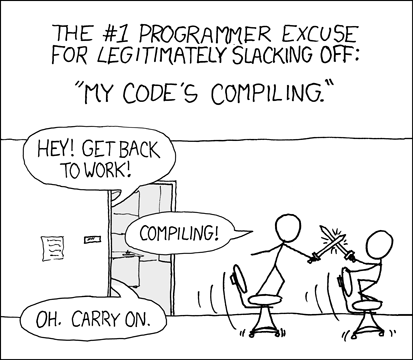
\includegraphics[width=0.8\columnwidth,height=5cm,keepaspectratio]{img/compiling.png}
\end{center}

% %% %%%%%%%%%%%%%%%%%%%%%%%%%%%%%%%%%%%%%%%%%%%%%%%%%%%%%%%%%%
% step-6.tex
%
% Author:  Mauricio Matamoros
% License: MIT
%
% %% %%%%%%%%%%%%%%%%%%%%%%%%%%%%%%%%%%%%%%%%%%%%%%%%%%%%%%%%%%

%!TEX root = ../practica.tex
%!TEX root = ../references.bib

% CHKTEX-FILE 1
% CHKTEX-FILE 13
% CHKTEX-FILE 46

\subsection{Paso 6: Grabación y prueba}%
\label{sec:step6}
Una vez que el sistema termine de compilar, encontrará la imagen generada \texttt{.img} dentro del directorio \texttt{output/images} de \emph{buldroot}.
Notará que el archivo de imagen no pesa más de 300MB.
¡Así de pequeño es su sistema operativo embebido!

Proceda a grabar la imagen generada en una memoria microSD utilizando \href{https://etcher.balena.io/}{Balena Etcher} de la misma forma que ha grabado otras imágenes.
Alternativamente puede grabar la imagen utilizando \texttt{dd} si conoce la ruta de la misma en su sistema con el comando:

\begin{Verbatim}[gobble=1]
	# dd if=output/images/sdcard.img of=/dev/<memoriaSD> bs=10M status=progress
\end{Verbatim}

\noindent
La grabación no debería tomar más que unos segundos.

% \begin{wrapfigure}{r}{0.4\textwidth}
% 	\centering
% 	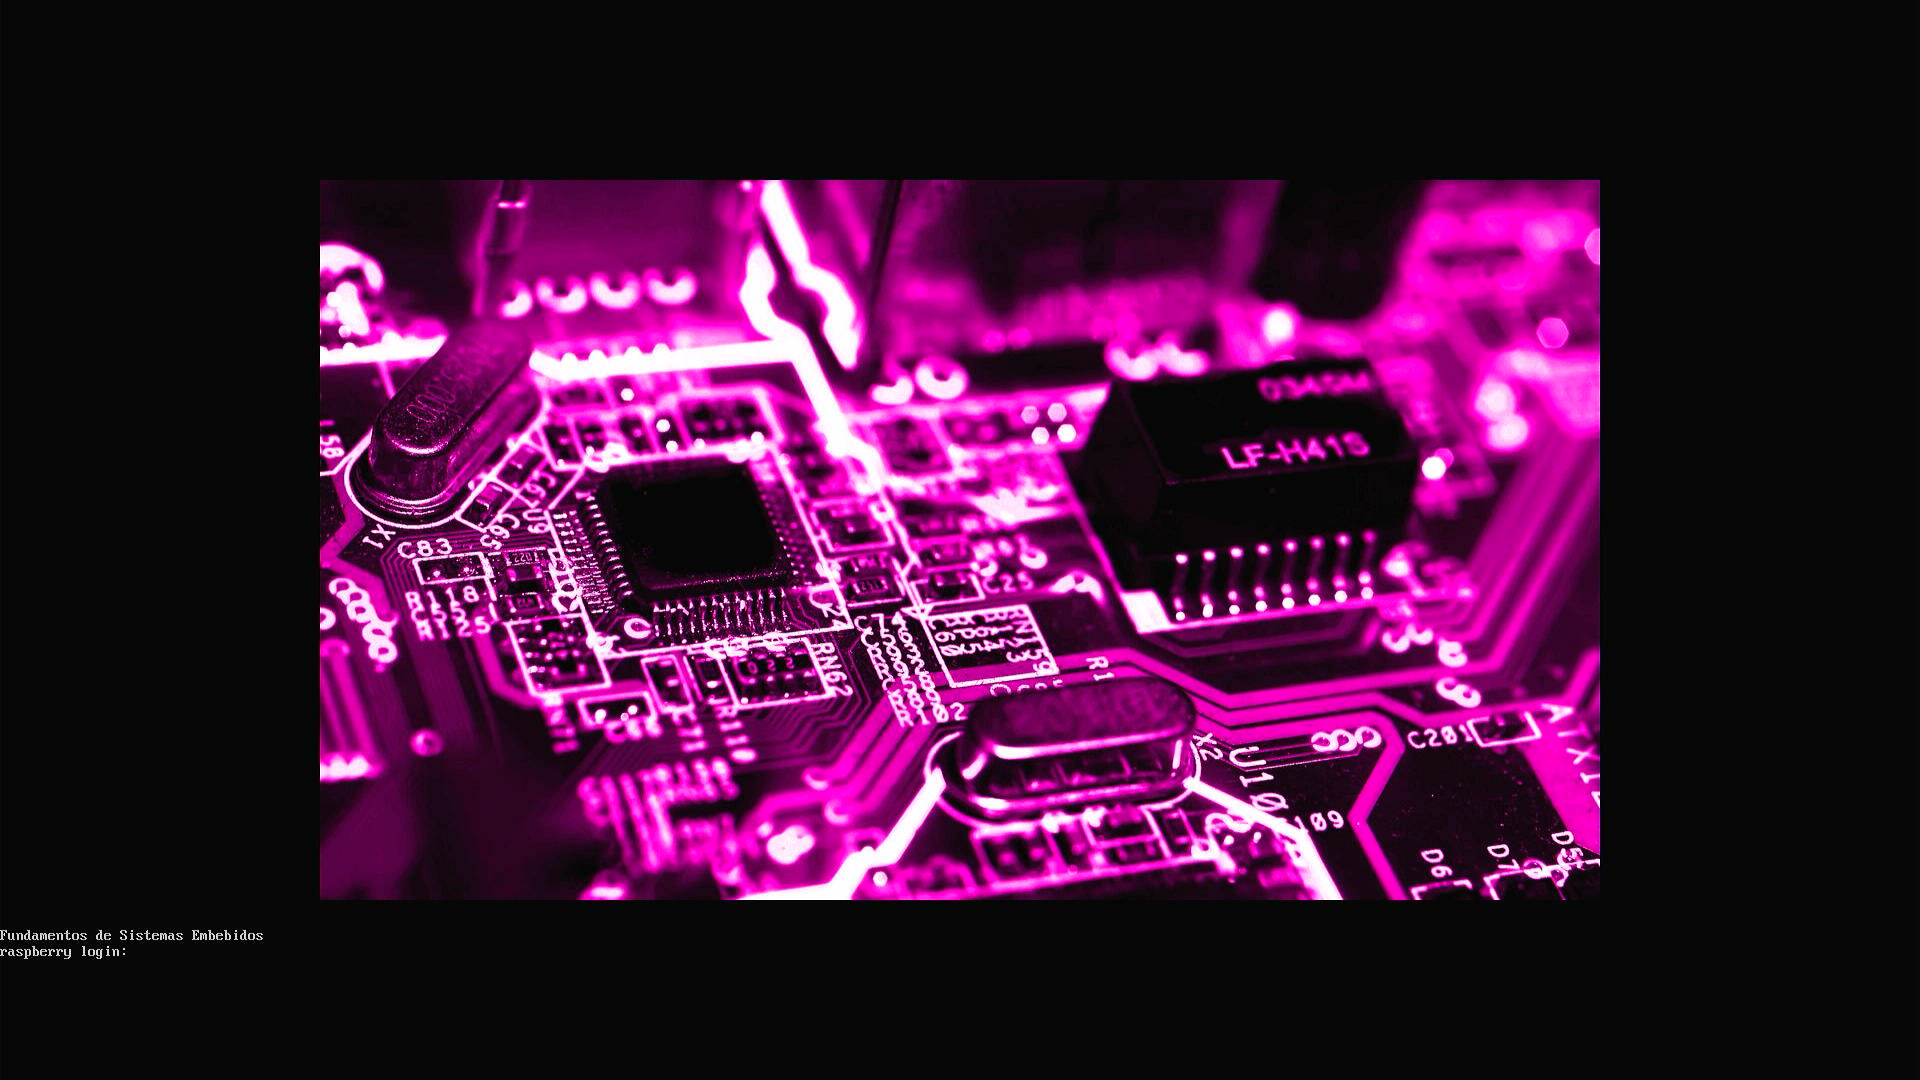
\includegraphics[width=0.38\textwidth]{img/system-running.jpg}
% \end{wrapfigure}
\begin{figure}
	\centering
	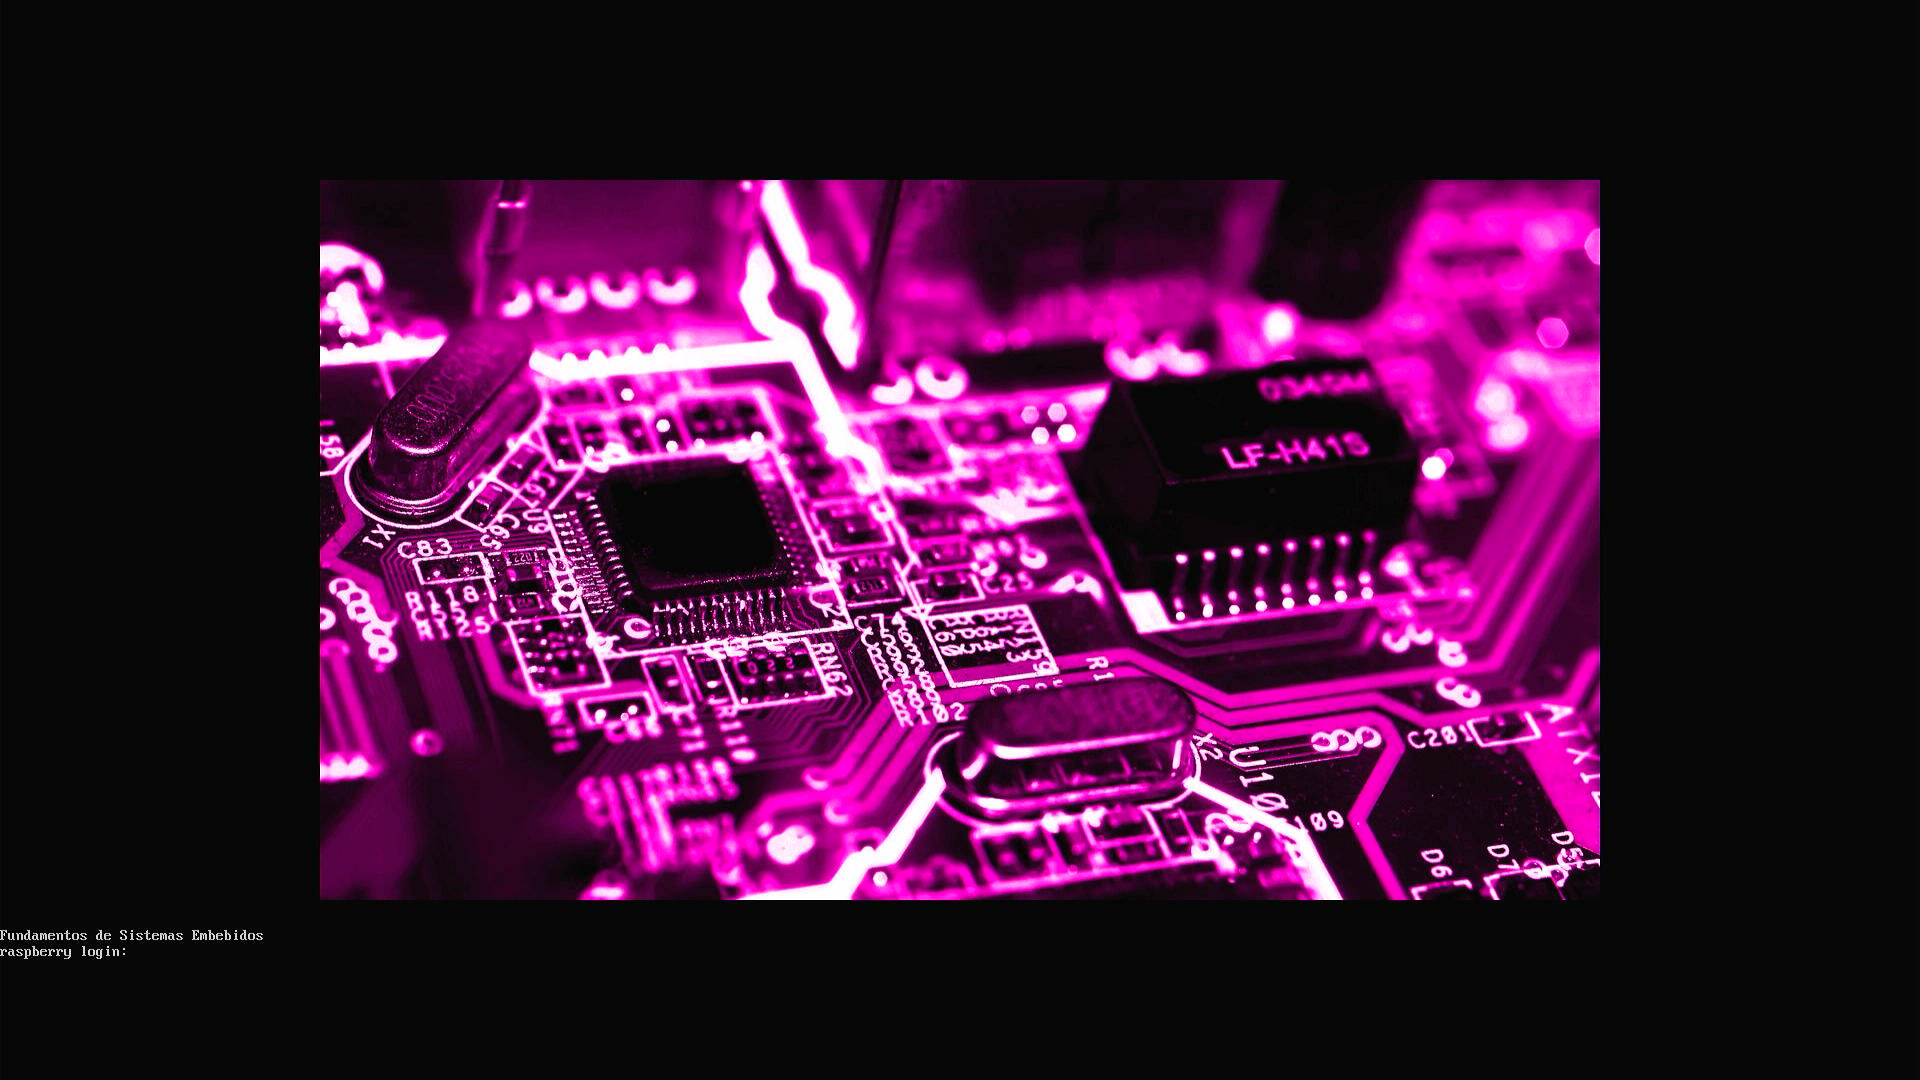
\includegraphics[width=0.8\textwidth,height=7cm,keepaspectratio]{img/system-running.jpg}
	\caption{Sistema embebido en ejecución con logotipo personalizado}%
	\label{fig:system-running}
\end{figure}
\medskip{}

Terminada la grabación, inserte la memoria microSD en la Raspberry Pi y observe el proceso de arranque, tendría que ver una pantalla similar a la de la~\Cref{fig:system-running}.
Cuando se lo solicite, inicie sesión con el usuario \texttt{pi} y la contraseña \texttt{raspberry}.


Conecte el display al puerto \IIC{} (pines 3 y 5 del puerto o GPIO2 y GPIO3 en BCM) y ejecute el comando de detección de dispositivos

\begin{Verbatim}[gobble=1]
	$ i2cdetect -y 1
\end{Verbatim}

\noindent
tendría que ver una salida como la siguiente:

\begin{Verbatim}[gobble=1]
	$ i2cdetect -y 1
	     0  1  2  3  4  5  6  7  8  9  a  b  c  d  e  f
	00:          -- -- -- -- -- -- -- -- -- -- -- -- --
	10: -- -- -- -- -- -- -- -- -- -- -- -- -- -- -- --
	20: -- -- -- -- -- -- -- 27 -- -- -- -- -- -- -- --
	30: -- -- -- -- -- -- -- -- -- -- -- -- -- -- -- --
	40: -- -- -- -- -- -- -- -- -- -- -- -- -- -- -- --
	50: -- -- -- -- -- -- -- -- -- -- -- -- -- -- -- --
	60: -- -- -- -- -- -- -- -- -- -- -- -- -- -- -- --
	70: -- -- -- -- -- -- -- --
\end{Verbatim}

